\section{Sensors}\label{sec:sensors}

The control system designed in the vessel requires the presence of sensor data that provide information about the vessel's motion. These are an Inertial Measurement Unit (IMU) and a Global Positioning System (GPS) module.

\subsection{IMU}

The Inertial Measurement Unit installed in the vessel is formed by a triaxial gyroscope with digital range scaling between ±75°/sec, ±150°/sec or ±300°/sec, a triaxial accelerometer with a range of ±18 g and a triaxial magnetometer with a range of ±\num{2.5} gauss. It also contains SPI-compatible serial interface to be able to obtain the data. \cite{IMUDatasheet}
%
\begin{figure}[H]
	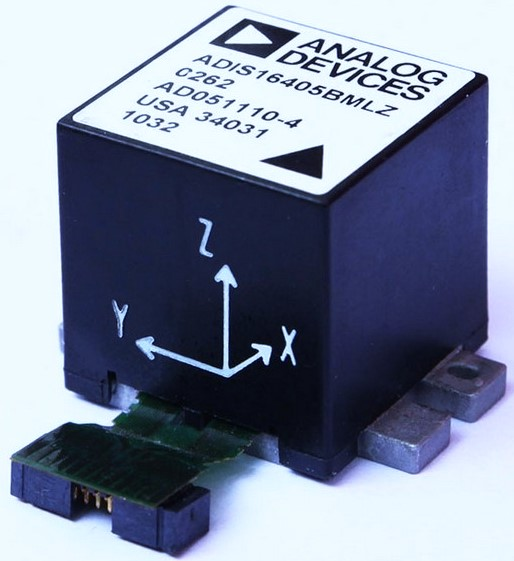
\includegraphics[width=0.3\textwidth]{figures/IMU}
	\caption{ADIS16405BMLZ IMU module mounted in the vessel \cite{IMUFigure}}
	\label{fig:IMU}
\end{figure}
%
The data provided by the IMU is used to estimate both the position and the attitude of the vessel and is extracted in the Low Level Interface through SPI serial communication.

%Triaxial, digital gyroscope with digital range scaling
%±75°/sec, ±150°/sec, ±300°/sec settings
%Tight orthogonal alignment, 0.05°
%Triaxial, digital accelerometer, ±18 g
%Triaxial, digital magnetometer, ±2.5 gauss
%SPI-compatible serial interface
%Embedded temperature sensor
%Single-supply operation: 4.75 V to 5.25 V

\subsection{GPS}
The vessel has a UP-501 GPS Receiver installed. It operates with a update frequency up to 10 Hz and its trasmits the received position data through a serial communication to the Low Level Interface. \cite{GPS}
%
\begin{figure}[H]
	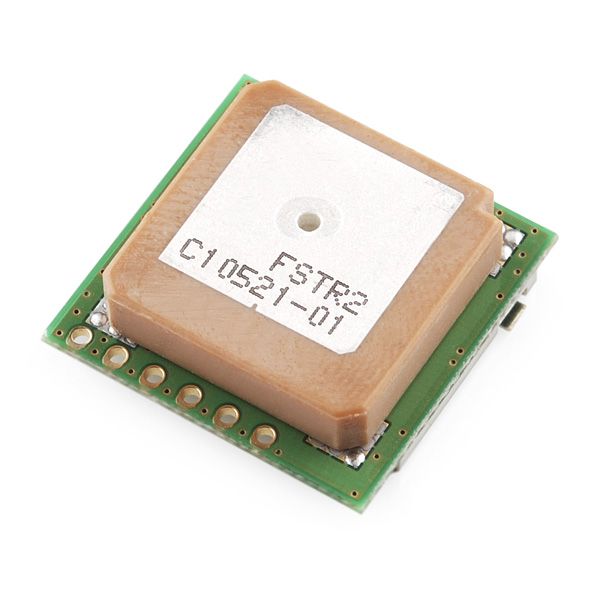
\includegraphics[width=0.3\textwidth]{figures/GPS}
	\caption{UP-501 GPS receiver mounted in the vessel \cite{GPS}.}
	\label{fig:GPS}
\end{figure}
%
As the UP-501 is a standard GPS receiver, its precision is in the range of meters \fxnote{How to prove this?? Maybe make a test.}. This makes it cumbersome to control the position of the vessel using only GPS data, and thus, the GPS and the IMU data is combined to obtained the position of the vessel.